% (find-LATEX "2021-1-C3-vetor-tangente.tex")
% (defun c () (interactive) (find-LATEXsh "lualatex -record 2021-1-C3-vetor-tangente.tex" :end))
% (defun C () (interactive) (find-LATEXsh "lualatex 2021-1-C3-vetor-tangente.tex" "Success!!!"))
% (defun D () (interactive) (find-pdf-page      "~/LATEX/2021-1-C3-vetor-tangente.pdf"))
% (defun d () (interactive) (find-pdftools-page "~/LATEX/2021-1-C3-vetor-tangente.pdf"))
% (defun e () (interactive) (find-LATEX "2021-1-C3-vetor-tangente.tex"))
% (defun o () (interactive) (find-LATEX "2021-1-C3-vetor-tangente.tex"))
% (defun u () (interactive) (find-latex-upload-links "2021-1-C3-vetor-tangente"))
% (defun v () (interactive) (find-2a '(e) '(d)))
% (defun d0 () (interactive) (find-ebuffer "2021-1-C3-vetor-tangente.pdf"))
% (defun cv () (interactive) (C) (ee-kill-this-buffer) (v) (g))
%          (code-eec-LATEX "2021-1-C3-vetor-tangente")
% (find-pdf-page   "~/LATEX/2021-1-C3-vetor-tangente.pdf")
% (find-sh0 "cp -v  ~/LATEX/2021-1-C3-vetor-tangente.pdf /tmp/")
% (find-sh0 "cp -v  ~/LATEX/2021-1-C3-vetor-tangente.pdf /tmp/pen/")
%     (find-xournalpp "/tmp/2021-1-C3-vetor-tangente.pdf")
%   file:///home/edrx/LATEX/2021-1-C3-vetor-tangente.pdf
%               file:///tmp/2021-1-C3-vetor-tangente.pdf
%           file:///tmp/pen/2021-1-C3-vetor-tangente.pdf
% http://angg.twu.net/LATEX/2021-1-C3-vetor-tangente.pdf
% (find-LATEX "2019.mk")
% (find-CN-aula-links "2021-1-C3-vetor-tangente" "3" "c3m211vt" "c3vt")
%
% «video»  	(to ".video")
% Video do semestre passado:
% (c3m202vta "video")

% Video novo (ainda não fiz):
% (find-ssr-links "c3m211vt" "2021-1-C3-vetor-tangente")
% (code-video     "c3m211vtvideo" "$S/http/angg.twu.net/eev-videos/2021-1-C3-vetor-tangente.mp4")
% (find-c3m211vtvideo "0:00")

% «.video»				(to "video")
% «.defs»				(to "defs")
% «.title»				(to "title")
% «.exercicio-1»			(to "exercicio-1")
% «.exercicio-2»			(to "exercicio-2")
% «.sobre-adivinhar-trajetorias»	(to "sobre-adivinhar-trajetorias")
% «.exercicio-3»			(to "exercicio-3")
% «.exercicio-4»			(to "exercicio-4")
%
% «.sympy»				(to "sympy")
% «.djvuize»				(to "djvuize")

\documentclass[oneside,12pt]{article}
\usepackage[colorlinks,citecolor=DarkRed,urlcolor=DarkRed]{hyperref} % (find-es "tex" "hyperref")
\usepackage{amsmath}
\usepackage{amsfonts}
\usepackage{amssymb}
\usepackage{pict2e}
\usepackage[x11names,svgnames]{xcolor} % (find-es "tex" "xcolor")
\usepackage{colorweb}                  % (find-es "tex" "colorweb")
%\usepackage{tikz}
%
% (find-dn6 "preamble6.lua" "preamble0")
%\usepackage{proof}   % For derivation trees ("%:" lines)
%\input diagxy        % For 2D diagrams ("%D" lines)
%\xyoption{curve}     % For the ".curve=" feature in 2D diagrams
%
\usepackage{edrx15}               % (find-LATEX "edrx15.sty")
\input edrxaccents.tex            % (find-LATEX "edrxaccents.tex")
\input edrxchars.tex              % (find-LATEX "edrxchars.tex")
\input edrxheadfoot.tex           % (find-LATEX "edrxheadfoot.tex")
\input edrxgac2.tex               % (find-LATEX "edrxgac2.tex")
%
%\usepackage[backend=biber,
%   style=alphabetic]{biblatex}            % (find-es "tex" "biber")
%\addbibresource{catsem-slides.bib}        % (find-LATEX "catsem-slides.bib")
%
% (find-es "tex" "geometry")
\usepackage[a6paper, landscape,
            top=1.5cm, bottom=.25cm, left=1cm, right=1cm, includefoot
           ]{geometry}
%
\begin{document}

%\catcode`\^^J=10
%\directlua{dofile "dednat6load.lua"}  % (find-LATEX "dednat6load.lua")

% %L dofile "edrxtikz.lua"  -- (find-LATEX "edrxtikz.lua")
% %L dofile "edrxpict.lua"  -- (find-LATEX "edrxpict.lua")
% \pu

% «defs»  (to ".defs")
% (find-LATEX "edrx15.sty" "colors-2019")
\long\def\ColorRed   #1{{\color{Red1}#1}}
\long\def\ColorViolet#1{{\color{MagentaVioletLight}#1}}
\long\def\ColorViolet#1{{\color{Violet!50!black}#1}}
\long\def\ColorGreen #1{{\color{SpringDarkHard}#1}}
\long\def\ColorGreen #1{{\color{SpringGreenDark}#1}}
\long\def\ColorGreen #1{{\color{SpringGreen4}#1}}
\long\def\ColorGray  #1{{\color{GrayLight}#1}}
\long\def\ColorGray  #1{{\color{black!30!white}#1}}
\long\def\ColorBrown #1{{\color{Brown}#1}}
\long\def\ColorBrown #1{{\color{brown}#1}}
\long\def\ColorOrange#1{{\color{orange}#1}}

\long\def\ColorShort #1{{\color{SpringGreen4}#1}}
\long\def\ColorLong  #1{{\color{Red1}#1}}

\def\frown{\ensuremath{{=}{(}}}
\def\True {\mathbf{V}}
\def\False{\mathbf{F}}
\def\D    {\displaystyle}

\def\drafturl{http://angg.twu.net/LATEX/2021-1-C3.pdf}
\def\drafturl{http://angg.twu.net/2021.1-C3.html}
\def\draftfooter{\tiny \href{\drafturl}{\jobname{}} \ColorBrown{\shorttoday{} \hours}}



%  _____ _ _   _                               
% |_   _(_) |_| | ___   _ __   __ _  __ _  ___ 
%   | | | | __| |/ _ \ | '_ \ / _` |/ _` |/ _ \
%   | | | | |_| |  __/ | |_) | (_| | (_| |  __/
%   |_| |_|\__|_|\___| | .__/ \__,_|\__, |\___|
%                      |_|          |___/      
%
% «title»  (to ".title")
% (c3m211vtp 1 "title")
% (c3m211vta   "title")

\thispagestyle{empty}

\begin{center}

\vspace*{1.2cm}

{\bf \Large Cálculo 3 - 2021.1}

\bsk

Aula 2: Vetores tangentes em $\R^2$

\bsk

Eduardo Ochs - RCN/PURO/UFF

\url{http://angg.twu.net/2021.1-C3.html}

\end{center}

\newpage

% Versão antiga:
% (c3m202vta "title")
% (c3m202vta "title" "Vetores tangentes em" "R^2")

{\bf Introdução}

Leia as páginas 187 a 199 do capítulo 6 do Bortolossi.

Nesta aula nós vamos representar curvas parametrizadas pelo
\ColorRed{traço} delas (p.188) com algumas anotações extras -- como
`$t=0$', `$t=1$', `$f(π)$' -- sobre pontos delas... além disso também
vamos desenhar vetores (vetores tangentes!) apoiados em alguns pontos,
fazer anotações neles também, e vamos usar tudo isso pra tentar
adivinhar (ééééé!) o comportamento de uma curva esquisita.

% (find-bortolossi6page (+ -186 188)   "traço")
% (find-bortolossi6page (+ -186 199)   "limite de vetores secantes")

\newpage

% «exercicio-1»  (to ".exercicio-1")
% (c3m211vtp 3 "exercicio-1")
% (c3m211vta   "exercicio-1")
% (c3m202vtp 3 "exercicio-1")
% (c3m202vt    "exercicio-1")

{\bf Exercício 1}

Sejam $P(t) = (4,0) + t\VEC{0,1}$ e $Q(u) = (0,3) + u\VEC{2,0}$.

Represente num gráfico só o traço de $P(t)$ e o de $Q(u)$.

Marque o ponto $P(0)$ e escreva `$t=0$' do lado dele.

Faça o mesmo para os pontos $P(1)$ (`$t=1$') e $Q(0)$ e $Q(1)$

(`$u=0$' e `$u=1$'). 

\msk

Seja $r$ o traço de $P(t)$ e $s$ o traço de $Q(u)$.

Seja $X$ o ponto de interseção de $r$ e $s$.

Quais são as coordenadas de $X$?

\msk

Cada ponto de $r$ está ``associado'' a um valor de $t$ e cada ponto de
$s$ a um valor de $u$. Quais são os valores de $t$ e $u$ associados ao
ponto $X$? Chame-os de $t_0$ e $u_0$ e indique-os no seu gráfico --
por exemplo, se $t_0=99$ e $u_0=200$ você vai escrever `$t=99$' e
`$u=200$' do lado do ponto $X$.

\newpage

{\bf Exercício 1 (continuação)}

Faça o desenho sozinho -- talvez você gaste alguns minutos pra
decifrar todas as instruções -- e depois compare o seu desenho com o
dos seus colegas.


\newpage

% «exercicio-2»  (to ".exercicio-2")
% (c3m211vtp 3 "exercicio-2")
% (c3m211vta   "exercicio-2")
% (c3m202vtp 5 "exercicio-2")
% (c3m202vt    "exercicio-2")

{\bf Exercício 2}

Seja $P(t) = (\cos t, \sen t)$.

Represente num gráfico só:

1) o traço de $P(t)$,

2) $P(\frac{π}{2}) + P'(\frac{π}{2})$, escrevendo `$P(\frac{π}{2})$'
ao lado do ponto

e `$P'(\frac{π}{2})$' ao lado da seta,

3) Idem para estes outros valores de $t$: $0, \frac14π, \frac34π, π$.

4) Seja $Q(u) = P(π) + uP'(π)$. Desenhe o traço de $Q(u)$ e anote
`$Q(0)$' e `$Q(1)$' nos pontos adequados.

\msk

5) O traço de $Q(u)$ é uma reta tangente ao traço de $P(t)$ no ponto
$P(π)$? Encontre no livro ou no resto da internet uma definição formal
de reta tangente e descubra se isto é verdade ou não.


\newpage

% «sobre-adivinhar-trajetorias»  (to ".sobre-adivinhar-trajetorias")
% (c3m211vtp 6 "sobre-adivinhar-trajetorias")
% (c3m211vta   "sobre-adivinhar-trajetorias")

{\bf Sobre ``adivinhar trajetórias''}

Nos próximos dois exercícios nós vamos {\sl começar} a fazer uma coisa
que vai ser muito comum aqui nesse curso de Cálculo 3, e que
geralmente é inadmissível nos cursos de Cálculo 1: nós vamos tentar
``advinhar'' como certas trajetórias são a partir de umas poucas
informações sobre elas.

Esse ``adivinhar'' na verdade é ``fazer hipóteses razoáveis'', e às
vezes a gente precisa de mais informações pra descobrir qual hipótese
é mais razoável. Na figura do próximo slide eu desenhei à esquerda
$P(t)+P'(t)$ para a trajetória de um personagem de videogame em
$t=0,1,3,4$, mas existem muitas trajetórias que se passam por esses
pontos com essas velocidades. Na primeira figura à direita eu desenhei
uma trajetória de uma nave no espaço; na segunda eu desenhei a
trajetória de um personagem de um videogame do meu tempo --- naquela
época nada nos videogames obedecia as leis da Física, e nos meus jogos
preferidos o meu personagem era um quadradinho --- e na terceira o
personagem é atingido por um raio em $t=1.05$ e ele adquire
superpoderes.

\bsk

% (find-latexscan-links "C3" "20210618_trajetorias")
% (find-xpdf-page "~/LATEX/2021-1-C3/20210618_trajetorias.pdf")
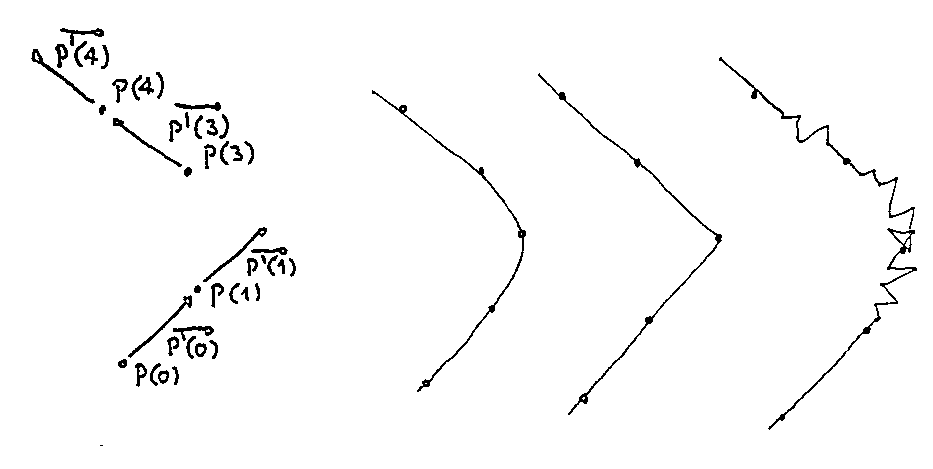
\includegraphics[height=6cm]{2021-1-C3/20210618_trajetorias.pdf}

\newpage

% «exercicio-3»  (to ".exercicio-3")
% (c3m211vtp 8 "exercicio-3")
% (c3m211vta   "exercicio-3")
% (c3m202vtp 6 "exercicio-3")
% (c3m202vt    "exercicio-3")

\vspace*{-0.75cm}

{\bf Exercício 3}

Seja $P(t) = (\cos t, \sen \ColorRed{2}t)$.

Represente graficamente $P(t)+P'(t)$ para os seguintes valores de $t$:

$0, \frac14π, \frac24π, \frac34π, \ldots, 2π$.

Faça as anotações adequadas nos seu pontos e vetores pra lembrar qual
é o $t$ associado a cada um.

\msk

\ColorRed{Tente} usar as informações deste gráfico pra desenhar o
traço de $P(t)$. Isto não é nada óbvio -- se inspire nas figuras das
páginas 208 e 209 do capítulo 6 do Bortolossi e tente conseguir uma
hipótese razoável.

\msk

Você pode pensar que $P(t)$ é a posição do Super Mario Kart no
instante $t$ e $P'(t)$ é o {\sl vetor velocidade} dele no instante $t$
(lembre que um vetor tem ``direção'', ``orientação'' e ``módulo''!)...
você só sabe a posição e a velocidade dele em alguns instantes, isto
é, em alguns valores de $t$, e você vai ter que encontrar uma
aproximação razoável, olhométrica, pra pista onde ele está correndo.



\newpage

% «exercicio-4»  (to ".exercicio-4")
% (c3m211vtp 9 "exercicio-4")
% (c3m211vta   "exercicio-4")
% (c3m201vtp 8 "exercicio-4")
% (c3m201vt    "exercicio-4")

{\bf Exercício 4}

Seja $P(t) = (\cos \ColorRed{2}t, \sen t)$.

Represente graficamente $P(t)+P'(t)$ para os seguintes valores de $t$:

$0, \frac14π, \frac24π, \frac34π, \ldots, 2π$.

Faça as anotações adequadas nos seu pontos e vetores pra lembrar qual
é o $t$ associado a cada um.

\msk

\ColorRed{Tente} usar as informações deste gráfico pra desenhar o
traço de $P(t)$. Isto não é nada óbvio -- se inspire nas figuras das
páginas 208 e 209 do capítulo 6 do Bortolossi e tente conseguir uma
hipótese razoável.


\msk

%\ColorRed{Obs: este exercício é bem mais fácil do que o 3! Eu deveria
%  ter apresentado ele antes do outro, mas acabei trocando a ordem por
%  um erro de digitação...}







%\printbibliography

\GenericWarning{Success:}{Success!!!}  % Used by `M-x cv'

\end{document}

% «sympy»  (to ".sympy")
% (c3m211vta "sympy")
% (c3m211vta "sympy" "Exercicio 4")

 (eepitch-vterm)
 (eepitch-kill)
 (eepitch-vterm)
isympy3
ee_dofile("~/.sympyrc.py")   # (find-angg ".sympyrc.py")
tpv = lambda t0: (t0, P.subs(t, t0), P.diff(t).subs(t, t0))

# Exercicio 2:
P = V2(cos(t), sin(t))
tpv(0)
tpv(pi/2)
tpv(pi)

# Exercicio 3: figura tipo um infinito
P = V2(cos(t), sin(2*t))
tpv(0)
tpv(pi/2)
tpv(pi)

# Exercicio 4: figura tipo um ")"
P = V2(cos(2*t), sin(t))
tpv(0)
tpv(pi/2)
tpv(pi)



%  ____  _             _         
% |  _ \(_)_   ___   _(_)_______ 
% | | | | \ \ / / | | | |_  / _ \
% | |_| | |\ V /| |_| | |/ /  __/
% |____// | \_/  \__,_|_/___\___|
%     |__/                       
%
% «djvuize»  (to ".djvuize")
% (find-LATEXgrep "grep --color -nH --null -e djvuize 2020-1*.tex")

 (eepitch-shell)
 (eepitch-kill)
 (eepitch-shell)
# (find-fline "~/2021.1-C3/")
# (find-fline "~/LATEX/2021-1-C3/")
# (find-fline "~/bin/djvuize")

cd /tmp/
for i in *.jpg; do echo f $(basename $i .jpg); done

f () { rm -fv $1.png $1.pdf; djvuize $1.pdf }
f () { rm -fv $1.png $1.pdf; djvuize WHITEBOARDOPTS="-m 1.0" $1.pdf; xpdf $1.pdf }
f () { rm -fv $1.png $1.pdf; djvuize WHITEBOARDOPTS="-m 0.5" $1.pdf; xpdf $1.pdf }
f () { rm -fv $1.png $1.pdf; djvuize WHITEBOARDOPTS="-m 0.25" $1.pdf; xpdf $1.pdf }
f () { cp -fv $1.png $1.pdf       ~/2021.1-C3/
       cp -fv        $1.pdf ~/LATEX/2021-1-C3/
       cat <<%%%
% (find-latexscan-links "C3" "$1")
%%%
}

f 20210618_trajetorias

f 20201213_area_em_funcao_de_theta
f 20201213_area_em_funcao_de_x
f 20201213_area_fatias_pizza



%  __  __       _        
% |  \/  | __ _| | _____ 
% | |\/| |/ _` | |/ / _ \
% | |  | | (_| |   <  __/
% |_|  |_|\__,_|_|\_\___|
%                        
% <make>

 (eepitch-shell)
 (eepitch-kill)
 (eepitch-shell)
# (find-LATEXfile "2019planar-has-1.mk")
make -f 2019.mk STEM=2021-1-C3-vetor-tangente veryclean
make -f 2019.mk STEM=2021-1-C3-vetor-tangente pdf

% Local Variables:
% coding: utf-8-unix
% ee-tla: "c3vt"
% ee-tla: "c3m211vt"
% End:
